\documentclass{pset}

\usepackage{xcolor}
\usepackage{amsmath}
\usepackage{tikz}
\usepackage{mathdots}
\usepackage{yhmath}
\usepackage{cancel}
\usepackage{siunitx}
\usepackage{array}
\usepackage{multirow}
\usepackage{amssymb}
\usepackage{gensymb}
\usepackage{tabularx}
\usepackage{booktabs}
\usetikzlibrary{fadings}
\usetikzlibrary{patterns}
\usetikzlibrary{shadows.blur}


\usepackage{hyperref}

\definecolor{hintpink}{RGB}{219, 48, 122}


\course{IrMO Combinatorics}
\name{Adam Kelly}
\due{\today}

 \blurb{\textbf{Remark.} This is a collection of all combinatorics problems that have appeared in the Irish Mathematical Olympiad and the Irish EGMO selection test.
 The questions are ordered chronologically. All problems are due to their respective creators.}


\newenvironment{hint}% environment name
{% begin code
\color{hintpink}
\noindent
  \begin{itshape}\textbf{Hint:}%
}%
{\end{itshape}}% end code

\begin{document}

\section*{EGMO Selection Test Problems}

\begin{problems}

\begin{problem}[EGMO TST 2020]
    Alice and Bob play the following game. 2020 coins are placed on a table. The players take turns, each removing either one or two coins in a turn. The player to remove the last coin loses. Bob goes first. Which of the two players has a strategy that is guaranteed to win?
\end{problem}

\begin{problem}[EGMO TST 2020]
    A pond has 2020 lily pads arranged in a circle. At time zero, two frogs (Anthony and Clare) share the same lily pad.

    Every minute, Anthony jumps over 99 lily pads in an anti-clockwise direction, to land on a pad 100 removed from where the jump started. At the same time, Clare jumps over 100 lily pads in a clockwise direction, to land on a pad 101 removed from where the jump started. What is the first time that Anthony and Clare are again within five lily pads of each other?
\end{problem}

\begin{problem}[EGMO TST 2019]
    The edges of a cube are coloured with three colours such that each vertex has exactly one edge of each of the three colours. Show that there are four parallel edges of the same colour.
\end{problem}

\begin{problem}[EGMO TST 2019]
    Let \(S\) be a set of \(6 n\) points on a line. \(4 n\) of these points are painted blue and the other \(2 n\) points are painted green.

    Prove that there exists a line segment that contains exactly \(3 n\) points from \(S\), such that \(2 n\) of them are blue and the other \(n\) are green.
\end{problem}

\begin{problem}[EGMO TST 2018]
    Emma writes the numbers \(1,2,3, \ldots, 9\) into the cells of a \(3 \times 3\) table (placing a different number in each cell). Then, she performs a series of moves as follows. In each move, she chooses an arbitrary \(2 \times 2\) square of the table, and either increases by 1 or else decreases by 1 all four numbers of that square. After performing a sequence of moves, Emma notices that all 9 numbers in the table are equal to some number \(n .\) Find, with proof, all possible values of \(n\)
\end{problem}

\begin{problem}[EGMO TST 2018]
    Let \(\mathcal{S}\) be a set of 2018 points in the plane, no three of which are collinear. Let \(P\) be a point not contained in any line segment that connects two points from \(\mathcal{S} .\) Prove that the number of triangles that contain \(P,\) with vertices at three different points in \(\mathcal{S},\) is even.
\end{problem}

\begin{problem}[EGMO TST 2017]
    Alice and Bob play a game with a string of 2017 pearls. In each move, one player cuts the string between two pearls and the other player chooses one of the resulting parts of the string while the other part is discarded. In the first move, Alice cuts the string. Thereafter, the players take turns. A player loses if he or she obtains a string with a single pearl such that no more cuts are possible. Which of the two players has a winning strategy?
\end{problem}

\begin{problem}[EGMO TST 2016]
    Consider the hexagon shown below. Alternately, two players play the following game: in one move one player
    selects one edge and colours it red and then the other player selects one remaining edge and colours it green. The winner is the player to complete first a triangle in their colour.
    \begin{center}
        \tikzset{every picture/.style={line width=0.75pt}} %set default line width to 0.75pt        

        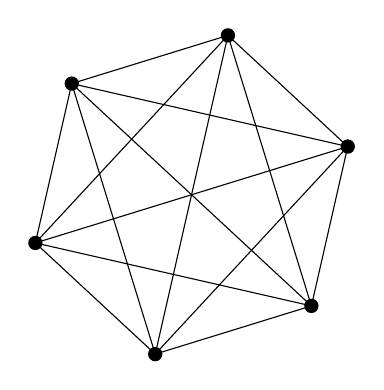
\begin{tikzpicture}[x=0.75pt,y=0.75pt,yscale=-0.75,xscale=0.75]
        %uncomment if require: \path (0,264); %set diagram left start at 0, and has height of 264

        %Shape: Regular Polygon [id:dp15342238181458812] 
        \draw   (240.33,92.04) -- (216.98,194.41) -- (116.65,225.37) -- (39.67,153.96) -- (63.02,51.59) -- (163.35,20.63) -- cycle ;
        %Straight Lines [id:da5727084142468732] 
        \draw    (63.02,51.59) -- (116.65,225.37) ;
        %Straight Lines [id:da02586682144860064] 
        \draw    (163.35,20.63) -- (216.98,194.41) ;
        %Straight Lines [id:da007527116532755507] 
        \draw    (216.98,194.41) -- (63.02,51.59) ;
        %Straight Lines [id:da5665703977595993] 
        \draw    (63.02,51.59) -- (240.33,92.04) ;
        %Straight Lines [id:da9506444299671366] 
        \draw    (39.67,153.96) -- (216.98,194.41) ;
        %Straight Lines [id:da3150074677220447] 
        \draw    (39.67,153.96) -- (240.33,92.04) ;
        %Straight Lines [id:da2886166022598726] 
        \draw    (39.67,153.96) -- (163.35,20.63) ;
        %Straight Lines [id:da7129544259234983] 
        \draw    (116.65,225.37) -- (163.35,20.63) ;
        %Straight Lines [id:da04190511424310839] 
        \draw    (116.65,225.37) -- (240.33,92.04) ;
        %Shape: Circle [id:dp5594723174040643] 
        \draw  [draw opacity=0][fill={rgb, 255:red, 0; green, 0; blue, 0 }  ,fill opacity=1 ] (112.05,225.37) .. controls (112.05,222.83) and (114.11,220.77) .. (116.65,220.77) .. controls (119.19,220.77) and (121.25,222.83) .. (121.25,225.37) .. controls (121.25,227.91) and (119.19,229.97) .. (116.65,229.97) .. controls (114.11,229.97) and (112.05,227.91) .. (112.05,225.37) -- cycle ;
        %Shape: Circle [id:dp9826422817463785] 
        \draw  [draw opacity=0][fill={rgb, 255:red, 0; green, 0; blue, 0 }  ,fill opacity=1 ] (212.38,194.41) .. controls (212.38,191.87) and (214.44,189.81) .. (216.98,189.81) .. controls (219.52,189.81) and (221.58,191.87) .. (221.58,194.41) .. controls (221.58,196.95) and (219.52,199.01) .. (216.98,199.01) .. controls (214.44,199.01) and (212.38,196.95) .. (212.38,194.41) -- cycle ;
        %Shape: Circle [id:dp4970273509008951] 
        \draw  [draw opacity=0][fill={rgb, 255:red, 0; green, 0; blue, 0 }  ,fill opacity=1 ] (235.73,92.04) .. controls (235.73,89.5) and (237.79,87.44) .. (240.33,87.44) .. controls (242.87,87.44) and (244.93,89.5) .. (244.93,92.04) .. controls (244.93,94.58) and (242.87,96.64) .. (240.33,96.64) .. controls (237.79,96.64) and (235.73,94.58) .. (235.73,92.04) -- cycle ;
        %Shape: Circle [id:dp21542310395401354] 
        \draw  [draw opacity=0][fill={rgb, 255:red, 0; green, 0; blue, 0 }  ,fill opacity=1 ] (158.75,20.63) .. controls (158.75,18.09) and (160.81,16.03) .. (163.35,16.03) .. controls (165.89,16.03) and (167.95,18.09) .. (167.95,20.63) .. controls (167.95,23.17) and (165.89,25.23) .. (163.35,25.23) .. controls (160.81,25.23) and (158.75,23.17) .. (158.75,20.63) -- cycle ;
        %Shape: Circle [id:dp20841448935128049] 
        \draw  [draw opacity=0][fill={rgb, 255:red, 0; green, 0; blue, 0 }  ,fill opacity=1 ] (58.42,51.59) .. controls (58.42,49.05) and (60.48,46.99) .. (63.02,46.99) .. controls (65.56,46.99) and (67.62,49.05) .. (67.62,51.59) .. controls (67.62,54.13) and (65.56,56.19) .. (63.02,56.19) .. controls (60.48,56.19) and (58.42,54.13) .. (58.42,51.59) -- cycle ;
        %Shape: Circle [id:dp5883482207845843] 
        \draw  [draw opacity=0][fill={rgb, 255:red, 0; green, 0; blue, 0 }  ,fill opacity=1 ] (35.07,153.96) .. controls (35.07,151.42) and (37.13,149.36) .. (39.67,149.36) .. controls (42.21,149.36) and (44.27,151.42) .. (44.27,153.96) .. controls (44.27,156.5) and (42.21,158.56) .. (39.67,158.56) .. controls (37.13,158.56) and (35.07,156.5) .. (35.07,153.96) -- cycle ;
        \end{tikzpicture}
    \end{center}
    Show that the player who goes first has a strategy that will always guarantee a win in four moves.
\end{problem}

\begin{problem}[EGMO TST 2016]
    25 boys and 25 girls are at a party. Each boy likes at least 13 girls, and each girl likes at least 13 boys.
    Show that there must be a boy and girl at the party who like each other.
\end{problem}

\begin{problem}[EGMO TST 2016]
    Richard and nine other people are standing in a circle. All ten of them think of an integer (that may be negative) and whisper their number to both of their neighbours. Afterwards, they each state the average of the two numbers that were whispered in their ear.

    Richard states the number \(10,\) his right neighbour states the number \(9,\) the next person along the circle states the number \(8,\) and so on, finishing with Richard's left neighbour who states the number 1
    What number did Richard have in mind?
\end{problem}

\begin{problem}[EGMO TST 2015]
    We have a deck of \(10,000\) cards, numbered from 1 to \(10,000 .\) A step consists of removing every card which has a perfect square on it, and then renumbering the remaining cards, starting from 1, in a consecutive way (i.e., numbering them \(1,2,3,\) etc. ) Find, with proof, the number of steps needed to remove all but one card.
\end{problem}

\begin{problem}[EGMO TST 2014]
    Show that for any integer \(n \geq 1\) we have
    $$
    \binom{n}{0}^2 + \binom{n}{1}^2 + \binom{n}{2}^2 + \cdots + \binom{n}{n}^2 = \binom{2n}{n}
    $$
\end{problem}

\begin{problem}[EGMO TST 2014]
    Let \(j, n\) be two integers such that \(n \geq 1\) and \(0 \leq j \leq n .\) Prove that
    $$
\sum_{k = j}^n \binom{n}{k} \binom{k}{j} = 2^{n - j} \binom{n}{j}
    $$
\end{problem}

\begin{problem}[EGMO TST 2013]
    Ciara and Emma are two of the ten students from which a team of five is to be selected for the next mathematical talent competition. In how many ways can a team of five students be formed so that Emma is on the team but Ciara is not?
\end{problem}

\begin{problem}[EGMO TST 2013]
    We are given a set \(X\) containing 100 integers, none of which is divisible by \(3 .\) We are asked to carry out the following task: choose 7 integers from this set so that for any pair of integers \(x\) and \(y\) we choose, the difference \(x-y\) is not divisible by \(9 .\)
    \begin{enumerate}
        \item Prove that this task is impossible.
        \item If we are instead asked to choose 6 integers from $X$, is the task always possible?
    \end{enumerate}
\end{problem}

\begin{problem}[EGMO TST 2013]
    In a deck of 52 cards, on each card there is a letter (one of $A$, $B$, $C$, $D$) and a number
    (between 1 and 13 inclusive). A poker hand consists of 5 cards from the deck (the ordering of the cards does not matter). Answer the following questions, justifying carefully your answer in each case. You may use the notation $\binom{n}{r}$ in your answers.
    \begin{enumerate}
        \item How many poker hands are there?
        \item How many poker hands do not have a card with a \(7 ?\)
        \item How many poker hands have (at least) two cards with the same letter?
        \item In how many poker hands does every letter appear?
    \end{enumerate}
\end{problem}

\begin{problem}[EGMO TST 2013]
    There are several people at a party. Any two people who are not friends with each other have exactly two friends in common. Anna and Brian are friends with each other, but don't have any friends in common. Show that Anna and Brian have the same number of friends at the party.
\end{problem}

\begin{problem}[EGMO TST 2012]
    Suppose 251 numbers are chosen from $1$, $2$, $3$, $\dots$, $499$, $500$. Show that, no matter how the numbers are chosen, there must be two that are consecutive.
\end{problem}

\begin{problem}[EGMO TST 2012]
    Suppose that \(a\) and \(m\) are integers larger than \(1 .\) Prove that the greatest common divisor of the pair \(a-1\) and \(m\) is equal to the greatest common divisor of the pair of integers \(a-1\) and \(\left(a^{m}-1\right) /(a-1)\)
\end{problem}

\begin{problem}[EGMO TST 2012]
    Seven darts are thrown at a circular dartboard of radius \(10 \mathrm{cm} .\) Show that there will always be two darts that are at most \(10 \mathrm{cm}\) apart.
\end{problem}

\begin{problem}[EGMO TST 2012]
    A set \(\mathcal{A}\) consists of 7 consecutive positive integers less than \(50,\) while another set \(\mathcal{B}\) consists
    of 11 consecutive positive integers. If the sum of the numbers in \(\mathcal{A}\) is equal to the sum of the numbers in \(\mathcal{B},\) what is the maximum possible element which could be contained in
    \(\mathcal{A} ?\)
\end{problem}

\end{problems}

\clearpage
\section*{IrMO Problems}

\begin{problems}


\begin{problem}[IrMO 2020 Q6]
    Pat has a pentagon, each of whose vertices is coloured either red or blue. Once an hour, Pat recolours the vertices as follows.
    \begin{itemize}
        \item Any vertex whose two neighbours were the same colour for the last hour, becomes blue for the next hour.
        \item Any vertex whose two neighbours were different colours for the last hour, becomes red for the next hour.
    \end{itemize}
Show that there is at least one vertex which is blue after the first recolouring and remains blue for ever.
\end{problem}

\begin{problem}[IrMO 2020 Q2]
    A round table has $2 N$ chairs around it. Due to social distancing guidelines, no two people are allowed to sit next to each other. How many different ways are there to choose seats around the table on which $N-1$ guests can be scated?
\end{problem}

\begin{problem}[IrMO 2019 Q2]
    Jenny is going to attend a sports camp for 7 days. Each day, she will play exactly one of three sports: hockey, tennis or camogie. The only restriction is that in any period of 4 consecutive days, she must play all three sports.
    Find, with proof, the number of possible sports schedules for Jennys week.
\end{problem}

\begin{problem}[IrMO 2019 Q10]
    Island Hopping Holidays offer short holidays to 64 islands, labeled Island \(i, 1 \leq i \leq\)
    64. A guest chooses any Island \(a\) for the first night of the holiday, moves to Island
    \(b\) for the second night, and finally moves to Island \(c\) for the third night. Due to the limited number of boats, we must have \(b \in T_{a}\) and \(c \in T_{b},\) where the sets \(T_{i}\) are chosen so that
    \begin{enumerate}
        \item each \(T_{i}\) is non-empty, and \(i \notin T_{i}\)
        \item \(\sum_{i=1}^{64}\left|T_{i}\right|=128,\) where \(\left|T_{i}\right|\) is the number of elements of \(T_{i}\)
    \end{enumerate}
    Exhibit a choice of sets \(T_{i}\) giving at least \(63 \cdot 64+6=4038\) possible holidays.
\end{problem}

\begin{problem}[IrMO 2018 Q4]
    We say that a rectangle with side lengths \(a\) and \(b\) fits inside a rectangle with side lengths \(c\) and \(d\) if either \((a \leq c \text { and } b \leq d)\) or \((a \leq d \text { and } b \leq c) .\) For instance, a rectangle with side lengths 1 and 5 fits inside a rectangle with side lengths 6 and 2 . Suppose \(S\) is a set of 2019 rectangles, all with integer side lengths between 1 and 2018 inclusive. Show that there are three rectangles \(A, B,\) and \(C\) in \(S\) such that \(A\) fits inside \(B,\) and \(B\) fits inside \(C .\)
\end{problem}

\begin{problem}[IrMO 2018 Q10]
    The game of Greed starts with an initial configuration of one or more piles of stones. Player 1 and Player 2 take turns to remove stones, beginning with Player 1. At each turn, a player has two choices:
    \begin{itemize}
        \item take one stone from any one of the piles (a simple move);
        \item take one stone from each of the remaining piles (a greedy move);
    \end{itemize}
    The player who takes the last stone wins. Consider the following two initial configurations:
    \begin{enumerate}
        \item There are 2018 piles, with either 20 or 18 stones in each pile.
        \item There are four piles, with 17, 18, 19 and 20 stones, respectively.
    \end{enumerate}
    In each case, find an appropriate strategy that guarentees victory to one of the players.
\end{problem}

\begin{problem}[IrMO 2017 Q4]
    An equilateral triangle of integer side length \(n \geq 1\) is subdivided into small triangles of unit side length, as illustrated in the figure below for the case \(n=5 .\) In this diagram, a subtriangle is a triangle of any size which is formed by connecting vertices of the small triangles along the grid-lines.
    \begin{center}
\tikzset{every picture/.style={line width=0.75pt}} %set default line width to 0.75pt        

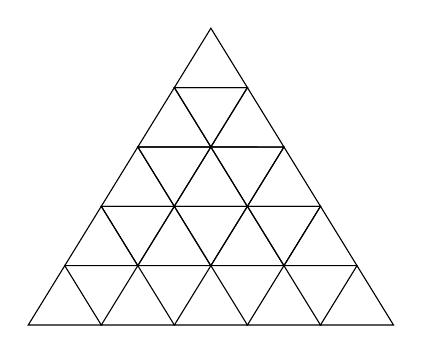
\begin{tikzpicture}[x=0.75pt,y=0.75pt,yscale=-0.5,xscale=0.5]
%uncomment if require: \path (0,704); %set diagram left start at 0, and has height of 704

%Shape: Triangle [id:dp13955414069322725] 
\draw   (264,22) -- (299.2,79.2) -- (228.8,79.2) -- cycle ;
%Shape: Triangle [id:dp0018918735078372606] 
\draw   (264,136.4) -- (228.8,79.2) -- (299.2,79.2) -- cycle ;
%Shape: Triangle [id:dp4387620141410302] 
\draw   (299.2,79.2) -- (334.4,136.4) -- (264,136.4) -- cycle ;
%Shape: Triangle [id:dp8181927792014567] 
\draw   (228.8,79.2) -- (264,136.4) -- (193.6,136.4) -- cycle ;
%Shape: Triangle [id:dp2722525906630253] 
\draw   (193.6,136.4) -- (228.8,193.6) -- (158.4,193.6) -- cycle ;
%Shape: Triangle [id:dp41006533113898525] 
\draw   (193.6,250.8) -- (158.4,193.6) -- (228.8,193.6) -- cycle ;
%Shape: Triangle [id:dp006559512064361783] 
\draw   (228.8,193.6) -- (264,250.8) -- (193.6,250.8) -- cycle ;
%Shape: Triangle [id:dp33101668856828437] 
\draw   (158.4,193.6) -- (193.6,250.8) -- (123.2,250.8) -- cycle ;
%Shape: Triangle [id:dp9561683055363637] 
\draw   (334.4,136.4) -- (369.6,193.6) -- (299.2,193.6) -- cycle ;
%Shape: Triangle [id:dp5130306280158132] 
\draw   (334.4,250.8) -- (299.2,193.6) -- (369.6,193.6) -- cycle ;
%Shape: Triangle [id:dp1932382913848938] 
\draw   (369.6,193.6) -- (404.8,250.8) -- (334.4,250.8) -- cycle ;
%Shape: Triangle [id:dp02090951403058705] 
\draw   (299.2,193.6) -- (334.4,250.8) -- (264,250.8) -- cycle ;
%Shape: Triangle [id:dp5142723962664604] 
\draw   (263.85,250.86) -- (228.73,193.63) -- (299.12,193.69) -- cycle ;
%Shape: Triangle [id:dp9529607962723157] 
\draw   (264,136.46) -- (299.13,193.69) -- (228.73,193.63) -- cycle ;
%Shape: Triangle [id:dp9050052873721142] 
\draw   (228.73,193.63) -- (193.6,136.4) -- (264,136.46) -- cycle ;
%Shape: Triangle [id:dp3860992745253269] 
\draw   (299.13,193.69) -- (264,136.46) -- (334.4,136.52) -- cycle ;
%Shape: Triangle [id:dp6201488609640171] 
\draw   (123.2,250.8) -- (158.4,308) -- (88,308) -- cycle ;
%Shape: Triangle [id:dp1969075316123805] 
\draw   (193.6,250.8) -- (228.8,308) -- (158.4,308) -- cycle ;
%Shape: Triangle [id:dp3233532254302558] 
\draw   (264,250.8) -- (299.2,308) -- (228.8,308) -- cycle ;
%Shape: Triangle [id:dp5277772230572277] 
\draw   (334.4,250.8) -- (369.6,308) -- (299.2,308) -- cycle ;
%Shape: Triangle [id:dp7618414210398883] 
\draw   (404.8,250.8) -- (440,308) -- (369.6,308) -- cycle ;
\end{tikzpicture}
    \end{center}
    It is desired to colour each vertex of the small triangles either red or blue in such a way that there is no subtriangle with all three of its vertices having the same colour. Let \(f(n)\) denote the number of distinct colourings satisfying this condition.

    Determine, with proof, $f(n)$ for every $n \geq 1$.
\end{problem}

\begin{problem}[IrMO 2017 Q7]
    Five teams play in a soccer competition where each team plays one match against each of the other four teams. A winning team gains 5 points and a losing team 0 points. For a \(0-0\) draw both teams gain 1 point, and for other draws \((1-1,2-2, \text { etc. })\) both teams gain 2 points. At the end of the competition, we write down the total points for each team, and we find that they form five consecutive integers. What is the minimum number of goals scored?
\end{problem}

\begin{problem}[IrMO 2014 Q1]
    Given an \(8 \times 8\) chess board, in how many ways can we select 56 squares on the board while satisfying both of the following requirements:
    \begin{enumerate}
        \item All black squares are selected.
        \item Exactly seven squares are selected in each column and in each row.
    
    \end{enumerate}
\end{problem}

\begin{problem}[IrMO 2014 Q10]
    Over a period of \(k\) consecutive days, a total of 2014 babies were born in a certain city, with at least one baby being born each day. Show that:
    \begin{enumerate}
        \item If \(1014<k \leq 2014,\) there must be a period of consecutive days during which exactly 100 babies were born.
        \item By contrast, if \(k=1014,\) such a period might not exist.    
    \end{enumerate}
\end{problem}

\begin{problem}[IrMO 2013 Q4]
    Each of the 36 squares of a \(6 \times 6\) table is to be coloured either Red, Yellow or Blue.
    \begin{itemize}
        \item No row or column is contain more than two squares of the same colour.
    \item In any four squares obtained by intersecting two rows with two columns, no colour is to occur exactly three times.
    \end{itemize}
    In how many different ways can the table be coloured if both of these rules are to
    be respected?
\end{problem}

\begin{problem}[IrMO 2013 Q7]
    Consider the collection of different squares which may be formed by sets of four points chosen from the 12 labelled points in the diagram below.

    \begin{center}
                 

\tikzset{every picture/.style={line width=0.75pt}} %set default line width to 0.75pt        

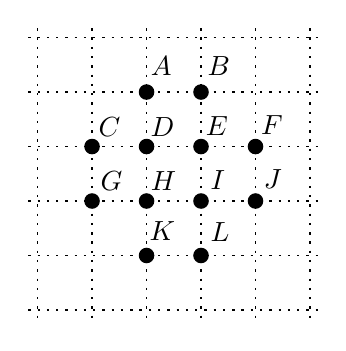
\begin{tikzpicture}[x=0.75pt,y=0.75pt,yscale=-0.75,xscale=0.75]
%uncomment if require: \path (0,704); %set diagram left start at 0, and has height of 704

%Shape: Grid [id:dp7714569274733274] 
\draw  [draw opacity=0][dash pattern={on 0.84pt off 2.51pt}] (100,63.6) -- (286,63.6) -- (286,252.6) -- (100,252.6) -- cycle ; \draw  [dash pattern={on 0.84pt off 2.51pt}] (106,63.6) -- (106,252.6)(141,63.6) -- (141,252.6)(176,63.6) -- (176,252.6)(211,63.6) -- (211,252.6)(246,63.6) -- (246,252.6)(281,63.6) -- (281,252.6) ; \draw  [dash pattern={on 0.84pt off 2.51pt}] (100,69.6) -- (286,69.6)(100,104.6) -- (286,104.6)(100,139.6) -- (286,139.6)(100,174.6) -- (286,174.6)(100,209.6) -- (286,209.6)(100,244.6) -- (286,244.6) ; \draw  [dash pattern={on 0.84pt off 2.51pt}]  ;
%Shape: Circle [id:dp305226010905727] 
\draw  [draw opacity=0][fill={rgb, 255:red, 0; green, 0; blue, 0 }  ,fill opacity=1 ] (171,104.6) .. controls (171,101.84) and (173.24,99.6) .. (176,99.6) .. controls (178.76,99.6) and (181,101.84) .. (181,104.6) .. controls (181,107.36) and (178.76,109.6) .. (176,109.6) .. controls (173.24,109.6) and (171,107.36) .. (171,104.6) -- cycle ;
%Shape: Circle [id:dp645562495221008] 
\draw  [draw opacity=0][fill={rgb, 255:red, 0; green, 0; blue, 0 }  ,fill opacity=1 ] (206,104.6) .. controls (206,101.84) and (208.24,99.6) .. (211,99.6) .. controls (213.76,99.6) and (216,101.84) .. (216,104.6) .. controls (216,107.36) and (213.76,109.6) .. (211,109.6) .. controls (208.24,109.6) and (206,107.36) .. (206,104.6) -- cycle ;
%Shape: Circle [id:dp11263874585797518] 
\draw  [draw opacity=0][fill={rgb, 255:red, 0; green, 0; blue, 0 }  ,fill opacity=1 ] (136,139.6) .. controls (136,136.84) and (138.24,134.6) .. (141,134.6) .. controls (143.76,134.6) and (146,136.84) .. (146,139.6) .. controls (146,142.36) and (143.76,144.6) .. (141,144.6) .. controls (138.24,144.6) and (136,142.36) .. (136,139.6) -- cycle ;
%Shape: Circle [id:dp21161811146798137] 
\draw  [draw opacity=0][fill={rgb, 255:red, 0; green, 0; blue, 0 }  ,fill opacity=1 ] (171,139.6) .. controls (171,136.84) and (173.24,134.6) .. (176,134.6) .. controls (178.76,134.6) and (181,136.84) .. (181,139.6) .. controls (181,142.36) and (178.76,144.6) .. (176,144.6) .. controls (173.24,144.6) and (171,142.36) .. (171,139.6) -- cycle ;
%Shape: Circle [id:dp17094367212240114] 
\draw  [draw opacity=0][fill={rgb, 255:red, 0; green, 0; blue, 0 }  ,fill opacity=1 ] (206,139.6) .. controls (206,136.84) and (208.24,134.6) .. (211,134.6) .. controls (213.76,134.6) and (216,136.84) .. (216,139.6) .. controls (216,142.36) and (213.76,144.6) .. (211,144.6) .. controls (208.24,144.6) and (206,142.36) .. (206,139.6) -- cycle ;
%Shape: Circle [id:dp49803305958672706] 
\draw  [draw opacity=0][fill={rgb, 255:red, 0; green, 0; blue, 0 }  ,fill opacity=1 ] (241,139.6) .. controls (241,136.84) and (243.24,134.6) .. (246,134.6) .. controls (248.76,134.6) and (251,136.84) .. (251,139.6) .. controls (251,142.36) and (248.76,144.6) .. (246,144.6) .. controls (243.24,144.6) and (241,142.36) .. (241,139.6) -- cycle ;
%Shape: Circle [id:dp08474553433829968] 
\draw  [draw opacity=0][fill={rgb, 255:red, 0; green, 0; blue, 0 }  ,fill opacity=1 ] (136,174.6) .. controls (136,171.84) and (138.24,169.6) .. (141,169.6) .. controls (143.76,169.6) and (146,171.84) .. (146,174.6) .. controls (146,177.36) and (143.76,179.6) .. (141,179.6) .. controls (138.24,179.6) and (136,177.36) .. (136,174.6) -- cycle ;
%Shape: Circle [id:dp8540286058534874] 
\draw  [draw opacity=0][fill={rgb, 255:red, 0; green, 0; blue, 0 }  ,fill opacity=1 ] (171,174.6) .. controls (171,171.84) and (173.24,169.6) .. (176,169.6) .. controls (178.76,169.6) and (181,171.84) .. (181,174.6) .. controls (181,177.36) and (178.76,179.6) .. (176,179.6) .. controls (173.24,179.6) and (171,177.36) .. (171,174.6) -- cycle ;
%Shape: Circle [id:dp6358026764884721] 
\draw  [draw opacity=0][fill={rgb, 255:red, 0; green, 0; blue, 0 }  ,fill opacity=1 ] (206,174.6) .. controls (206,171.84) and (208.24,169.6) .. (211,169.6) .. controls (213.76,169.6) and (216,171.84) .. (216,174.6) .. controls (216,177.36) and (213.76,179.6) .. (211,179.6) .. controls (208.24,179.6) and (206,177.36) .. (206,174.6) -- cycle ;
%Shape: Circle [id:dp306138036268508] 
\draw  [draw opacity=0][fill={rgb, 255:red, 0; green, 0; blue, 0 }  ,fill opacity=1 ] (241,174.6) .. controls (241,171.84) and (243.24,169.6) .. (246,169.6) .. controls (248.76,169.6) and (251,171.84) .. (251,174.6) .. controls (251,177.36) and (248.76,179.6) .. (246,179.6) .. controls (243.24,179.6) and (241,177.36) .. (241,174.6) -- cycle ;
%Shape: Circle [id:dp7647430845733172] 
\draw  [draw opacity=0][fill={rgb, 255:red, 0; green, 0; blue, 0 }  ,fill opacity=1 ] (171,209.6) .. controls (171,206.84) and (173.24,204.6) .. (176,204.6) .. controls (178.76,204.6) and (181,206.84) .. (181,209.6) .. controls (181,212.36) and (178.76,214.6) .. (176,214.6) .. controls (173.24,214.6) and (171,212.36) .. (171,209.6) -- cycle ;
%Shape: Circle [id:dp8392922513675309] 
\draw  [draw opacity=0][fill={rgb, 255:red, 0; green, 0; blue, 0 }  ,fill opacity=1 ] (206,209.6) .. controls (206,206.84) and (208.24,204.6) .. (211,204.6) .. controls (213.76,204.6) and (216,206.84) .. (216,209.6) .. controls (216,212.36) and (213.76,214.6) .. (211,214.6) .. controls (208.24,214.6) and (206,212.36) .. (206,209.6) -- cycle ;

% Text Node
\draw (185.5,87.67) node    {$A$};
% Text Node
\draw (222.5,88) node    {$B$};
% Text Node
\draw (152.17,127) node    {$C$};
% Text Node
\draw (186.17,127) node    {$D$};
% Text Node
\draw (221.17,126.33) node    {$E$};
% Text Node
\draw (256.5,126) node    {$F$};
% Text Node
\draw (153.5,161.67) node    {$G$};
% Text Node
\draw (186.83,161.67) node    {$H$};
% Text Node
\draw (221.83,161) node    {$I$};
% Text Node
\draw (257.17,160.67) node    {$J$};
% Text Node
\draw (186.17,194) node    {$K$};
% Text Node
\draw (223.17,194.33) node    {$L$};


\end{tikzpicture}
   
    \end{center}
            
    For each possible area such a square may have, determine the number of squares which have this area.
    
    Make sure to explain why your list is complete.
\end{problem}

\begin{problem}[IrMO 2012 Q1]
    Let
    $$
    C=\{1,2,3,4,5,6,7,8,9,10,11,12,13,14,16,17,18,19,20\}
    $$
    and let
    $$
    S=\{4,5,9,14,23,37\}
    $$
    Find two sets \(A\) and \(B\) with the properties
    \begin{itemize}
    \item \(A \cap B=\emptyset\)
\item \(A \cup B=C\)
\item The sum of two distinct elements of \(A\) is not in \(S\).
\item The sum of two distinct elements of \(B\) is not in \(S\).
    \end{itemize}
\end{problem}

\begin{problem}[IrMO 2012 Q10]
    Let \(n\) be a positive integer. A mouse sits at each corner point of an \(n \times n\) square board, which is divided into unit squares.

    The mice then move according to a sequence of steps, in the following manner:
\begin{enumerate}
    \item  In each step, each of the four mice travels a distance of one unit in a horizontal
or vertical direction. Each unit distance is called an edge of the board, and we say that each mouse uses an edge of the board.
\item  An edge of the board may not be used twice in the same direction.
\item At most two mice may occupy the same point on the board at any time.
\end{enumerate}

The mice wish to collectively organise their movements so that each edge of the board will be used twice (not necessarily by the same mouse), and each mouse will finish up at its starting point. Determine, with proof, the values of \(n\) for which the mice may achieve this goal.
\end{problem}



\begin{problem}[IrMO 2011 Q5]
    In the mathematical talent show called ``The $X^2$-factor'' contestants are scored by a panel of 8 judges. Each judge awards a score of 0 (`fail'), $X$ (`pass'), or $X^2$ (`pass with distinction'). Three of the contestants were Ann, Barbara and David. Ann was awarded the same score as Barbara by exactly 4 of the judges. David declares that he obtained different scores to Ann from at least 4 of the judges, and also that he obtained different scores to Barbara from at least 4 judges.

    In how many ways could scores have been allocated to David, assuming he is telling the truth?
\end{problem}


\begin{problem}[IrMO 2011 Q6]
    In a tournament with \(N\) players, \(N<10,\) each player plays once against each other player scoring 1 point for a win and 0 points for a loss. Draws do not occur. In a particular tournament only one player ended with an odd number of points and was ranked fourth. Determine whether or not this is possible. If so, how many wins did the player have?
\end{problem}

\begin{problem}[IrMO 2010 Q4]
    The country of Harpland has three types of coin: green, white and orange. The unit of currency in Harpland is the shilling. Any coin is worth a positive integer number of shillings, but coins of the same colour may be worth different amounts.
    A set of coins is stacked in the form of an equilateral triangle of side \(n\) coins.

    The stacking has the following properties:
    \begin{enumerate}
        \item no coin touches another coin of the same colour;
        \item the total worth, in shillings, of the coins lying on any line parallel to one of the sides of the triangle is divisible by three.
    \end{enumerate}

Prove that the total worth in shillings of the green coins in the triangle is divisible by three.
\end{problem}

\begin{problem}[IrMO 2010 Q6]
    There are 14 boys in a class. Each boy is asked how many other boys in the class have his first name, and how many have his last name. It turns out that each number from 0 to 6 occurs among the answers.

    Prove that there are two boys in the class with the same first name and the same last name.
\end{problem}


\begin{problem}[IrMO 2009 Q1]
    Hamilton Avenue has eight houses. On one side of the street are the houses numbered \(1,3,5,7\) and directly opposite are houses \(2,4,6,8\) respectively. An eccentric postman starts deliveries at house 1 and delivers letters to each of the houses, finally returning to house 1 for a cup of tea. Throughout the entire journey he must observe the following rules. The numbers of the houses delivered to must follow an odd-even-odd-even pattern throughout, each house except house 1 is visited exactly once (house 1 is visited twice) and the postman at no time is allowed to cross the road to the house directly opposite. How many different delivery sequences are possible?
\end{problem}

\begin{problem}[IrMO 2009 Q4]
    Given an \(n\)-tuple of numbers \(\left(x_{1}, x_{2}, \ldots, x_{n}\right)\) where each \(x_{i}=+1\) or \(-1,\) form a new \(n\)-tuple
$$
\left(x_{1} x_{2}, x_{2} x_{3}, x_{3} x_{4}, \ldots, x_{n} x_{1}\right)
$$
and continue to repeat this operation. Show that if \(n=2^{k}\) for some integer \(k \geq 1\) then after a certain number of repetitions of the operation, we obtain the \(n\)-tuple
$$
(1,1,1, \ldots, 1)
$$

\end{problem}

\begin{problem}[IrMO 2009 Q9]
    At a strange party, each person knew exactly 22 others.
    For any pair of people \(X\) and \(Y\) who knew one another, there was no other person at the party that they both knew.
    
    For any pair of people \(X\) and \(Y\) who did not know one another, there were exactly
    6 other people that they both knew.
    How many people were at the party?
\end{problem}

\begin{problem}[IrMO 2008 Q4]
    How many sequences \(a_{1}, a_{2}, \ldots, a_{2008}\) are there such that each of the numbers
    \(1,2, \ldots, 2008\) occurs once in the sequence, and \(i \in\left\{a_{1}, a_{2}, \ldots, a_{i}\right\}\) for each \(i\) such that \(2 \leq i \leq 2008 ?\)
\end{problem}

\begin{problem}[IrMO 2008 Q9]
    Given \(k \in\{0,1,2,3\}\) and a positive integer \(n,\) let \(f_{k}(n)\) be the number of sequences \(x_{1}, \ldots, x_{n},\) where \(x_{i} \in\{-1,0,1\}\) for \(i=1, \ldots, n,\) and
    $$
    x_{1}+\cdots+x_{n} \equiv k \quad \bmod 4
    $$
    \begin{enumerate}
    \item Prove that \(f_{1}(n)=f_{3}(n)\) for all positive integers \(n\)
    \item Prove that
    $$
    f_{0}(n)=\frac{3^{n}+2+(-1)^{n}}{4}
    $$
    for all positive integers \(n\)
    \end{enumerate}
\end{problem}

\begin{problem}[IrMO 2007 Q4]
    Air Michael and Air Patrick operate direct flights connecting Belfast, Cork, Dublin, Galway, Limerick and Waterford. For each pair of cities exactly one of the airlines operates the route (in both directions) connecting the cities. Prove that there are four cities for which one of the airlines operates a round trip. (Note that a round trip of four cities \(P, Q, R\) and \(S,\) is a journey that follows the path \(P \rightarrow Q \rightarrow R \rightarrow S \rightarrow P .)\)
\end{problem}


\begin{problem}[IrMO 2006 Q6]
    The rooms of a building are arranged in a \(m \times n\) rectangular grid (as shown below for the \(5 \times 6\) case). Every room is connected by an open door to each adjacent room, but the only access to or from the building is by a door in the top right room. This door is locked with an elaborate system of \(m n\) keys, one of which is located in every room of the building. A person is in the bottom left room and can move from there to any adjacent room. However, as soon as the person leaves a room, all the doors of that room are instantly and automatically locked. Find, with proof, all \(m\) and \(n\) for which it is possible for the person to collect all the keys and escape the building.

    \begin{center}
        

\tikzset{every picture/.style={line width=0.75pt}} %set default line width to 0.75pt        

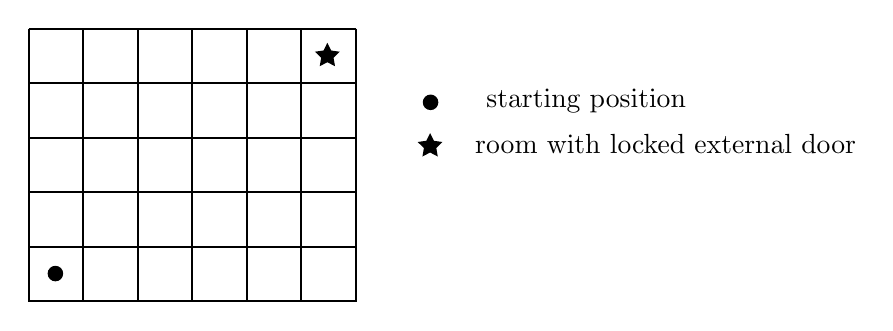
\begin{tikzpicture}[x=0.75pt,y=0.75pt,yscale=-0.75,xscale=0.75]
%uncomment if require: \path (0,704); %set diagram left start at 0, and has height of 704

%Shape: Grid [id:dp7874470792373589] 
\draw  [draw opacity=0][line width=0.75]  (74.86,111.31) -- (285.14,111.31) -- (285.14,286.94) -- (74.86,286.94) -- cycle ; \draw  [line width=0.75]  (74.86,111.31) -- (74.86,286.94)(109.86,111.31) -- (109.86,286.94)(144.86,111.31) -- (144.86,286.94)(179.86,111.31) -- (179.86,286.94)(214.86,111.31) -- (214.86,286.94)(249.86,111.31) -- (249.86,286.94)(284.86,111.31) -- (284.86,286.94) ; \draw  [line width=0.75]  (74.86,111.31) -- (285.14,111.31)(74.86,146.31) -- (285.14,146.31)(74.86,181.31) -- (285.14,181.31)(74.86,216.31) -- (285.14,216.31)(74.86,251.31) -- (285.14,251.31)(74.86,286.31) -- (285.14,286.31) ; \draw  [line width=0.75]   ;
%Shape: Circle [id:dp696078713003516] 
\draw  [draw opacity=0][fill={rgb, 255:red, 0; green, 0; blue, 0 }  ,fill opacity=1 ] (87,268.6) .. controls (87,265.84) and (89.24,263.6) .. (92,263.6) .. controls (94.76,263.6) and (97,265.84) .. (97,268.6) .. controls (97,271.36) and (94.76,273.6) .. (92,273.6) .. controls (89.24,273.6) and (87,271.36) .. (87,268.6) -- cycle ;
%Shape: Star [id:dp13903595514451772] 
\draw  [draw opacity=0][fill={rgb, 255:red, 0; green, 0; blue, 0 }  ,fill opacity=1 ] (266.71,120.33) -- (269.17,125.3) -- (274.67,126.09) -- (270.69,129.95) -- (271.63,135.41) -- (266.71,132.83) -- (261.79,135.41) -- (262.73,129.95) -- (258.74,126.09) -- (264.25,125.3) -- cycle ;
%Shape: Circle [id:dp39640302967260843] 
\draw  [draw opacity=0][fill={rgb, 255:red, 0; green, 0; blue, 0 }  ,fill opacity=1 ] (328,158.6) .. controls (328,155.84) and (330.24,153.6) .. (333,153.6) .. controls (335.76,153.6) and (338,155.84) .. (338,158.6) .. controls (338,161.36) and (335.76,163.6) .. (333,163.6) .. controls (330.24,163.6) and (328,161.36) .. (328,158.6) -- cycle ;
%Shape: Star [id:dp9640383383367526] 
\draw  [draw opacity=0][fill={rgb, 255:red, 0; green, 0; blue, 0 }  ,fill opacity=1 ] (332.71,178.33) -- (335.17,183.3) -- (340.67,184.09) -- (336.69,187.95) -- (337.63,193.41) -- (332.71,190.83) -- (327.79,193.41) -- (328.73,187.95) -- (324.74,184.09) -- (330.25,183.3) -- cycle ;

% Text Node
\draw (433,158) node   [align=left] {starting position};
% Text Node
\draw (484,185) node   [align=left] {room with locked external door};


\end{tikzpicture}

    \end{center}
\end{problem}

\begin{problem}[IrMO 2006 Q10]
    Two positive integers \(n\) and \(k\) are given, with \(n \geq 2 .\) In the plane there are \(n\) circles such that any two of them intersect at two points and all these intersection points are distinct. Each intersection point is coloured with one of \(n\) given colours in such
    a way that all \(n\) colours are used. Moreover, on each circle there are precisely \(k\)
    different colours present. Find all possible values for \(n\) and \(k\) for which such a colouring is possible.
\end{problem}

\begin{problem}[IrMO 2005 Q9]
    Determine the number of different arrangements \(a_{1}, a_{2}, \ldots, a_{10}\) of the integers \(1,2, \ldots, 10\) such that
    $$
    a_{i}>a_{2 i} \text { for } 1 \leq i \leq 5
    $$
    and
    $$
    a_{i}>a_{2 i+1} \text { for } 1 \leq i \leq 4
    $$
\end{problem}

\begin{problem}[IrMO 2004 Q2]
    Each of the players in a tennis tournament played one match against each of the others. If every player won at least one match, show that there is a group \(A, B, C\) of three players for which \(A\) beat \(B, B\) beat \(C\) and \(C\) beat \(A .\)
\end{problem}

\begin{problem}[IrMO 2003 Q4]
    Eight players, Ann, Bob, Con, Dot, Eve, Fay, Guy and Hal compete in a chess tournament. No pair plays together more than once and there is no group of five people in which each one plays against all of the other four.
    \begin{enumerate}
        \item Write down an arrangement for a tournament of 24 games satisfying these conditions.
        \item Show that it is impossible to have a tournament of more than 24 games satisfying these conditions.
    \end{enumerate}
\end{problem}

\begin{problem}[IrMO 2003 Q10]
    \begin{enumerate}
        \item In how many ways can 1003 distinct integers be chosen from the set \(\{1,2, \ldots, 2003\}\)
        so that no two of the chosen integers differ by \(10 ?\)
        \item Show that there are \((3(5151)+7(1700)) 101^{7}\) ways to choose 1002 distinct integers from the set \(\{1,2, \ldots, 2003\}\) so that no two of the chosen integers differ by \(10 .\)
    
    \end{enumerate}
    \end{problem}

\begin{problem}[IrMO 2002 Q2]
    \begin{enumerate}
    \item A group of people attends a party. Each person has at most three acquaintances in the group, and if two people do not know each other, then they have a mutual acquaintance in the group. What is the maximum number of people present?
    \item If, in addition, the group contains three mutual acquaintances (i.e., three people each of whom knows the other two), what is the maximum number of people?
    \end{enumerate}
\end{problem}

\begin{problem}[IrMO 2002 Q6]
    \(\mathrm{A} 3 \times n\) grid is filled as follows : the first row consists of the numbers from 1 to \(n\) arranged from left to right in ascending order. The second row is a cyclic shift of the top row. Thus the order goes \(i, i+1, \ldots, n-1, n, 1,2, \ldots, i-1\) for some \(i .\) The third row has the numbers 1 to \(n\) in some order, subject to the rule that in each of the \(n\) columns, the sum of the three numbers is the same.

    For which values of \(n\) is it possible to fill the grid according to the above rules? For an \(n\) for which this is possible, determine the number of different ways of filling the grid.
\end{problem}

\begin{problem}[IrMO 2001 Q7]
    Three hoops are arranged concentrically as in the diagram. Each hoop is threaded with 20 beads, of which 10 are black and 10 are white. On each hoop the positions of the beads are labelled 1 through 20 starting at the bottom and travelling counterclockwise.

    We say there is a match at position \(i\) if all three beads at position \(i\) have the same colour. We are free to slide all of the beads around any hoop (but not to unthread and rethread them).

    \begin{center}
        

\tikzset{every picture/.style={line width=0.75pt}} %set default line width to 0.75pt        

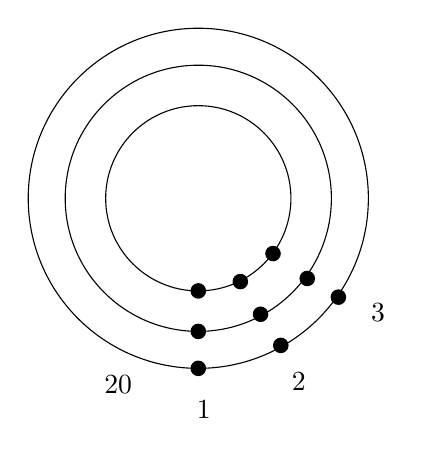
\begin{tikzpicture}[x=0.75pt,y=0.75pt,yscale=-0.75,xscale=0.75]
%uncomment if require: \path (0,704); %set diagram left start at 0, and has height of 704

%Shape: Circle [id:dp5122940331166459] 
\draw   (72,216.5) .. controls (72,183.64) and (98.64,157) .. (131.5,157) .. controls (164.36,157) and (191,183.64) .. (191,216.5) .. controls (191,249.36) and (164.36,276) .. (131.5,276) .. controls (98.64,276) and (72,249.36) .. (72,216.5) -- cycle ;
%Shape: Circle [id:dp39076554485495496] 
\draw   (46,216.5) .. controls (46,169.28) and (84.28,131) .. (131.5,131) .. controls (178.72,131) and (217,169.28) .. (217,216.5) .. controls (217,263.72) and (178.72,302) .. (131.5,302) .. controls (84.28,302) and (46,263.72) .. (46,216.5) -- cycle ;
%Shape: Circle [id:dp08744048135109028] 
\draw   (22.25,216.5) .. controls (22.25,156.16) and (71.16,107.25) .. (131.5,107.25) .. controls (191.84,107.25) and (240.75,156.16) .. (240.75,216.5) .. controls (240.75,276.84) and (191.84,325.75) .. (131.5,325.75) .. controls (71.16,325.75) and (22.25,276.84) .. (22.25,216.5) -- cycle ;
%Shape: Circle [id:dp5339051285104826] 
\draw  [draw opacity=0][fill={rgb, 255:red, 0; green, 0; blue, 0 }  ,fill opacity=1 ] (126.5,276) .. controls (126.5,273.24) and (128.74,271) .. (131.5,271) .. controls (134.26,271) and (136.5,273.24) .. (136.5,276) .. controls (136.5,278.76) and (134.26,281) .. (131.5,281) .. controls (128.74,281) and (126.5,278.76) .. (126.5,276) -- cycle ;
%Shape: Circle [id:dp08101394467600076] 
\draw  [draw opacity=0][fill={rgb, 255:red, 0; green, 0; blue, 0 }  ,fill opacity=1 ] (126.5,302) .. controls (126.5,299.24) and (128.74,297) .. (131.5,297) .. controls (134.26,297) and (136.5,299.24) .. (136.5,302) .. controls (136.5,304.76) and (134.26,307) .. (131.5,307) .. controls (128.74,307) and (126.5,304.76) .. (126.5,302) -- cycle ;
%Shape: Circle [id:dp11735720881726164] 
\draw  [draw opacity=0][fill={rgb, 255:red, 0; green, 0; blue, 0 }  ,fill opacity=1 ] (126.5,325.75) .. controls (126.5,322.99) and (128.74,320.75) .. (131.5,320.75) .. controls (134.26,320.75) and (136.5,322.99) .. (136.5,325.75) .. controls (136.5,328.51) and (134.26,330.75) .. (131.5,330.75) .. controls (128.74,330.75) and (126.5,328.51) .. (126.5,325.75) -- cycle ;
%Shape: Circle [id:dp9832102178999709] 
\draw  [draw opacity=0][fill={rgb, 255:red, 0; green, 0; blue, 0 }  ,fill opacity=1 ] (179.5,311) .. controls (179.5,308.24) and (181.74,306) .. (184.5,306) .. controls (187.26,306) and (189.5,308.24) .. (189.5,311) .. controls (189.5,313.76) and (187.26,316) .. (184.5,316) .. controls (181.74,316) and (179.5,313.76) .. (179.5,311) -- cycle ;
%Shape: Circle [id:dp016766926570799034] 
\draw  [draw opacity=0][fill={rgb, 255:red, 0; green, 0; blue, 0 }  ,fill opacity=1 ] (153.5,270) .. controls (153.5,267.24) and (155.74,265) .. (158.5,265) .. controls (161.26,265) and (163.5,267.24) .. (163.5,270) .. controls (163.5,272.76) and (161.26,275) .. (158.5,275) .. controls (155.74,275) and (153.5,272.76) .. (153.5,270) -- cycle ;
%Shape: Circle [id:dp15367520095446618] 
\draw  [draw opacity=0][fill={rgb, 255:red, 0; green, 0; blue, 0 }  ,fill opacity=1 ] (174.5,252) .. controls (174.5,249.24) and (176.74,247) .. (179.5,247) .. controls (182.26,247) and (184.5,249.24) .. (184.5,252) .. controls (184.5,254.76) and (182.26,257) .. (179.5,257) .. controls (176.74,257) and (174.5,254.76) .. (174.5,252) -- cycle ;
%Shape: Circle [id:dp785461937853789] 
\draw  [draw opacity=0][fill={rgb, 255:red, 0; green, 0; blue, 0 }  ,fill opacity=1 ] (166.5,291) .. controls (166.5,288.24) and (168.74,286) .. (171.5,286) .. controls (174.26,286) and (176.5,288.24) .. (176.5,291) .. controls (176.5,293.76) and (174.26,296) .. (171.5,296) .. controls (168.74,296) and (166.5,293.76) .. (166.5,291) -- cycle ;
%Shape: Circle [id:dp1545455522345267] 
\draw  [draw opacity=0][fill={rgb, 255:red, 0; green, 0; blue, 0 }  ,fill opacity=1 ] (196.5,268) .. controls (196.5,265.24) and (198.74,263) .. (201.5,263) .. controls (204.26,263) and (206.5,265.24) .. (206.5,268) .. controls (206.5,270.76) and (204.26,273) .. (201.5,273) .. controls (198.74,273) and (196.5,270.76) .. (196.5,268) -- cycle ;
%Shape: Circle [id:dp8121559679771104] 
\draw  [draw opacity=0][fill={rgb, 255:red, 0; green, 0; blue, 0 }  ,fill opacity=1 ] (216.5,280) .. controls (216.5,277.24) and (218.74,275) .. (221.5,275) .. controls (224.26,275) and (226.5,277.24) .. (226.5,280) .. controls (226.5,282.76) and (224.26,285) .. (221.5,285) .. controls (218.74,285) and (216.5,282.76) .. (216.5,280) -- cycle ;

% Text Node
\draw (80,336) node    {$20$};
% Text Node
\draw (135,352) node    {$1$};
% Text Node
\draw (196,334) node    {$2$};
% Text Node
\draw (247,290) node    {$3$};


\end{tikzpicture}

    \end{center}

    Show that it is possible (by sliding) to find a configuration involving at least 5 matches.
\end{problem}

\begin{problem}[IrMO 2000 Q4]
    Let \(a_{1}<a_{2}<a_{3}<\cdots<a_{M}\)
    be real numbers. \(\left\{a_{1}, a_{2}, \ldots, a_{M}\right\}\) is called a weak arithmetic progression of length \(M\) if there exist real numbers \(x_{0}, x_{1}, x_{2}, \ldots, x_{M}\) and \(d\) such that
    $$
    x_{0} \leq a_{1}<x_{1} \leq a_{2}<x_{2} \leq a_{3}<x_{3} \leq \cdots \leq a_{M}<x_{M}
    $$
    and for \(i=0,1,2, \ldots, M-1, x_{i+1}-x_{i}=d\) i.e. \(\left\{x_{0}, x_{1}, x_{2}, \ldots, x_{M}\right\}\) is an arithmetic
    progression.
    \begin{enumerate}
     \item Prove that if \(a_{1}<a_{2}<a_{3},\) then \(\left\{a_{1}, a_{2}, a_{3}\right\}\) is a weak arithmetic progression
    of length 3.
    \item Let \(A\) be a subset of \(\{0,1,2,3, \ldots, 999\}\) with at least 730 members. Prove that
    \(A\) contains a weak arithmetic progression of length \(10 .\)
\end{enumerate}
\end{problem}

\begin{problem}[IrMO 1999 Q4]
    A square floor consists of 10000 squares \((100 \text { squares } \times 100 \text { squares }-\) like a large chessboard) is to be tiled. The only available tiles are rectangular \(1 \times 3\) tiles, fitting exactly over three squares of the floor.
    \begin{enumerate}
    \item If a \(2 \times 2\) square is removed from the centre of the floor, prove that the remaining part of the floor can be tiles with the available tiles.
    \item If, instead, a \(2 \times 2\) square is removed from a corner of the floor, prove that the remaining part of the floor cannot be tiled with the available tiles.
\end{enumerate}
    
    [There are sufficiently many tiles available. To tile the floor - or a portion thereof
    - means to completely cover it with the tiles, each tile covering three squares, and no pair of tiles overlapping. The tiles may not be broken or cut.]
\end{problem}

\begin{problem}[IrMO 1998 Q8]
    Let \(\mathbb{N}\) be the set of all natural numbers (i.e., the positive integers).
    \begin{enumerate}
        \item Prove that \(\mathbb{N}\) can be written as a union of three mutually disjoint sets such that, if \(m, n \in \mathbb{N}\) and \(|m-n|=2\) or \(5,\) then \(m\) and \(n\) are in different sets.
    \item Prove that \(\mathbb{N}\) can be written as a union of four mutually disjoint sets such that, if \(m, n \in \mathbb{N}\) and \(|m-n|=2,3\) or \(5,\) then \(m\) and \(n\) are in different sets. Show, however, that it is impossible to write \(\mathbb{N}\) as a union of three mutually disjoint sets with this property.
    \end{enumerate}
    
\end{problem}

\begin{problem}[IrMO 1997 Q8]
    Let \(A\) be a subset of \(\{0,1,2,3, \ldots, 1997\}\) containing more than 1000 elements. Prove that either \(A\) contains a power of 2 (that is, a number of the form \(2^{k},\) with \(k\) a nonnegative integer) or there exist two distinct elements \(a, b \in A\) such that \(a+b\) is a power of 2
\end{problem}

\begin{problem}[IrMO 1997 Q9]
    Let \(S\) be the set of all natural numbers \(n\) satisfying the following conditions:
    \begin{enumerate}
    \item \(n\) has 1000 digits;
    \item all the digits of \(n\) are odd, and
    \item the absolute value of the difference between adjacent digits of \(n\) is \(2 .\)
\end{enumerate}
    Determine the number of distinct elements in \(S\).
\end{problem}

\begin{problem}[IrMO 1995 Q1]
    There are \(n^{2}\) students in a class. Each week all the students participate in a table quiz. Their teacher arranges them into \(n\) teams of \(n\) players each. For as many weeks as possible, this arrangement is done in such a way that any pair of students who were members of the same team one week are not on the same team in subsequent weeks. Prove that after at most \(n+2\) weeks, it is necessary for some pair of students to have been members of the same team on at least two different weeks.
\end{problem}

\begin{problem}[IrMO 1995 Q4]
    Consider the following one-person game played on the \(x\) -axis. For each integer \(k\)
    let \(X_{k}\) be the point with coordinates \((k, 0) .\) During the game discs are piled at some of the points \(X_{k} .\) To perform a move in the game, the player chooses a point
    \(X_{j}\) at which at least two discs are piled and then takes two discs from the pile at
    \(X_{j}\) and places one of them at \(X_{j-1}\) and one at \(X_{j+1}\)
    To begin the game, \(2 n+1\) discs are placed at \(X_{0} .\) The player then proceeds to perform moves in the game for as long as possible. Prove that after \(n(n+1)(2 n+1)/6\)
     moves no further moves are possible, and that, at this stage, one disc remains
    at each of the positions
    $$
    X_{-n}, X_{-n+1}, \ldots, X_{-1}, X_{0}, X_{1}, \ldots, X_{n-1}, X_{n}
    $$
\end{problem}

\begin{problem}[IrMO 1994 Q4]
    Consider the set of \(m \times n\) matrices with every entry either 0 or \(1 .\) Determine the number of such matrices with the property that the number of ``1''s in each row and in each column is even.
\end{problem}


\begin{problem}[IrMO 1994 Q10]
    If a square is partitioned into \(n\) convex polygons, determine the maximum number of edges present in the resulting figure.
\end{problem}

\begin{problem}[IrMO 1993 Q6]
    Given five points \(P_{1}, P_{2}, P_{3}, P_{4}, P_{5}\) in the plane having integer coordinates, prove that there is at least one pair \(\left(P_{i}, P_{j}\right),\) with \(i \neq j,\) such that the line \(P_{i} P_{j}\) contains a point \(Q\) having integer coordinates and lying strictly between \(P_{i}\) and \(P_{j}\).
\end{problem}

\begin{problem}[IrMO 1993 Q8]
Prove the identity
$$
\sum_{d = 1}^{\infty} \binom{n - r + 1}{d} \binom{r - 1}{d - 1} = \binom{n}{r}
$$
for all integers $n$ and $r$, with $1 \leq r \leq n$.
\end{problem}

\begin{problem}[IrMO 1993 Q10]
    \begin{enumerate}
    \item The rectangle \(P Q R S\) has \(|P Q|=\ell\) and \(|Q R|=m,\) where \(\ell, m\) are positive integers. It is divided up into \(\ell m 1 \times 1\) squares by drawing lines parallel to \(P Q\) and \(Q R .\) Prove that the diagonal \(P R\) intersects \(\ell+m-d\) of these squares, where \(d\) is the greatest common divisor, \((\ell, m),\) of \(\ell\) and \(m\)
    \item A cuboid (or box) with edges of lengths \(\ell, m, n,\) where \(\ell, m, n\) are positive integers, is divided into \(\ell m n 1 \times 1 \times 1\) cubes by planes parallel to its faces. Consider a diagonal joining a vertex of the cuboid to the vertex furthest away from it. How many of the cubes does this diagonal intersect?
\end{enumerate}
\end{problem}

\begin{problem}[IrMO 1992 Q3]
    Let \(A\) be a nonempty set with \(n\) elements. Find the number of ways of choosing a pair of subsets \((B, C)\) of \(A\) such that \(B\) is a nonempty subset of \(C\).
\end{problem}

\begin{problem}[IrMO 1993 Q3]
    Three operations \(f, g\) and \(h\) are defined on subsets of the natural numbers \(\mathbb{N}\) as follows:
    \begin{itemize}
        \item \(f(n)=10 n,\) if \(n\) is a positive integer; 
        \item \(g(n)=10 n+4,\) if \(n\) is a positive integer; 
        \item \(h(n)=\frac{n}{2},\) if \(n\) is an even positive integer.
    \end{itemize}
     Prove that, starting from \(4,\) every natural number can be constructed by performing a finite number of operations \(f, g\) and \(h\) in some order. [For example: $35=h(f(h(g(h(h(4)))))))$ .]
\end{problem}


\begin{problem}[IrMO 1991 Q4]
    Eight politicians stranded on a desert island on January lst, \(1991,\) decided to establish a parliment. They decided on the following rules of attendance:
    \begin{enumerate}
        \item There should always be at least one person present on each day.
        \item On no two days should be same subset attend.
        \item The members present on day \(N\) should include for each \(K<N,(K \geq 1)\) at least one member who was present on day \(K\)
    \end{enumerate}
    For how many days can the parliment sit before one of the rules is broken?
\end{problem}

\begin{problem}[IrMO 1990 Q1]
    Given a natural number \(n,\) calculate the number of rectangles in the plane, the coordinates of whose vertices are integers in the range 0 to \(n,\) and whose sides are parallel to the axes.
\end{problem}

\begin{problem}[IrMO 1990 Q9]
    Let \(n=2 k-1,\) where \(k \geq 6\) is an integer. Let \(T\) be the set of all \(n\)-tuples $$\mathbf{x}=\left(x_{1}, x_{2}, \ldots, x_{n}\right),$$ where, for \(i=1,2, \ldots, n, x_{i}\) is 0 or 1.

    For \(\mathbf{x}=\left(x_{1}, \ldots, x_{n}\right)\) and \(\mathbf{y}=\left(y_{1}, \ldots, y_{n}\right)\) in \(T,\) let \(d(\mathbf{x}, \mathbf{y})\) denote the number of integers \(j\) with \(1 \leq j \leq n\) such that \(x_{j} \neq y_{j} .\) (In particular, \(d(\mathbf{x}, \mathbf{x})=0\) ). 
    
    Suppose that there exists a subset \(S\) of \(T\) with \(2^{k}\) elements which has the following property: given any element \(\mathbf{x}\) in \(T,\) there is a unique \(\mathbf{y}\) in \(S\) with \(d(\mathbf{x}, \mathbf{y}) \leq 3\) 
    
    Prove that \(n=23\)
\end{problem}

\begin{problem}[IrMO 1989 Q7]
    Each of the \(n\) members of a club is given a different item of information. They are allowed to share the information, but, for security reasons, only in the following way: A pair may communicate by telephone. During a telephone call only one member may speak. The member who speaks may tell the other member all the information s(he) knows. Determine the minimal number of phone calls that are required to convey all the information to each other.
\end{problem}

\begin{problem}[IrMO 1988 Q5]
    A person has seven friends and invites a different subset of three friends to dinner every night for one week (seven days). In how many ways can this be done so that all friends are invited at least once?
\end{problem}

\begin{problem}[IrMO 1988 Q6]
    Suppose you are given \(n\) blocks, each of which weighs an integral number of pounds, but less than \(n\) pounds. Suppose also that the total weight of the \(n\) blocks is less than \(2 n\) pounds. Prove that the blocks can be divided into two groups, one of which weighs exactly \(n\) pounds.
\end{problem}

\begin{problem}[IrMO 1988 Q15]
    A city has a system of bus routes laid out in such a way that
    \begin{enumerate}
        \item there are exactly 11 bus stops on each route;
        \item it is possible to travel between any two bus stops without changing routes;
        \item any two bus routes have exactly one bus stop in common.
        What is the number of bus routes in the city?
    \end{enumerate}
\end{problem}







\end{problems}
\end{document}